Для того, чтобы протестировать разработанные алгоритмы, был реализован на языке программирования С++ класс RandomGraph, хранящий рёбра в списках смежности . Класс содержат в себе метод, который генерирует случайный граф по модели Эрдёша-Реньи. Для реализации этой модели использовалось случайная величина $\in R[0,1]$. 

Также RandomGraph содержит обязательную для нашей задачи проверку на связность. На основе этого класса реализован соответствующий класс алгоритмов, который содержит методы, ищущие решение задачи распространения информации в графе. Вершину-терминал, в которой изначально хранится информация, храним как поле класса.

Чтобы перейти к обобщениям задачи, достаточно вместо одной вершины-терминала хранить массив терминалов, в которых изначально находится информация. А чтобы перейти к ориентированному графу, строим ориентированный граф по модели Эрдёша-Реньи, которая незначительно отличается от изложенной выше модели (случайный эксперимент теперь проводим для дуги графа, их в 2 раза больше).

Весь код программы выложен в открытый доступ, с ним можно ознакомиться, протестировать, убедиться в его правильности. Ссылка:
\href{https://github.com/KlicOgogo/KlicAll/tree/master/Cpp/University/Course\%20project}{https://git hub.com/KlicOgogo/KlicAll/tree/master/Cpp/University/Course\%20project}
	
Перейдём к тестированию. Будем генерировать случайный граф, и на нём запускать все алгоритмы. В таблицы войдут результаты двадцати тестов, каждая таблица будет соответствовать группе алгоритмов, которые были описаны ранее.

Для рандомизированных алгоритмов с неоднократным повторением будем брать число максимальное число повторений, равное пяти.

Сначала протестируем наши алгоритмы на графе большого размера и достаточно большой вероятностью проведения ребра, чтобы получить достаточно плотный граф. Для этого возьмём в качестве параметров $n = 1000$, $p = 0.2$.

\setcounter{figure}{0}
\begin{table}[H]
	\begin{center}
		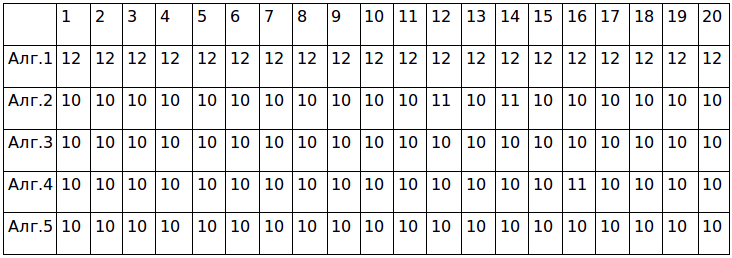
\includegraphics[scale=0.65]{table1.png}
		\caption{$n = 1000$, $p = 0.2$}
	\end{center}
\end{table}

Пользуясь утверждением 1, получаем, что минимальное число шагов, за которое можно распространить информацию, равно 10, а это значение было достигнуто всеми алгоритмами почти на всех тестах, кроме первого.

Теперь возьмём разреженный граф того же размера, для получения разреженности уменьшим вероятность проведения ребра в 20 раз, т.е. $p = 0.01$.

\begin{table}[H]
	\begin{center}
		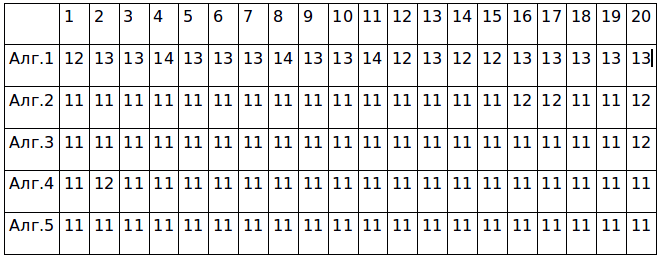
\includegraphics[scale=0.7]{table2.png}
		\caption{$n = 1000$, $p = 0.01$}
	\end{center}
\end{table}

Из результатов можно видеть, что на разреженных графах, сгенерированных моделью Эрдёша-Реньи, реализованные эвристики работают хорошо. Рассмотрим ещё граф средней плотности и протестируем на нём алгоритмы. Для этого сделаем $p = 0.1$, $n = 100$. 

\begin{table}[H]
	\begin{center}
		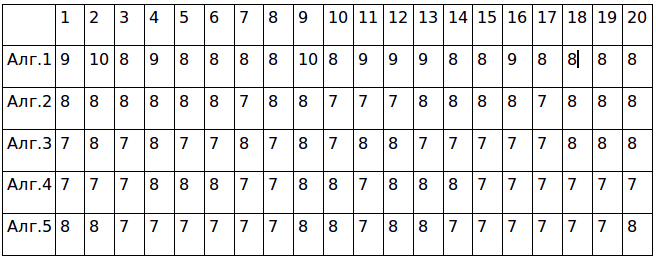
\includegraphics[scale=0.7]{table3.png}
		\caption{$n = 100$, $p = 0.1$}
	\end{center}
\end{table}
